%
% db.tex -- Daubechies wavelets als Beispiele
%
% (c) 2019 Prof Dr Andreas Müller, Hochschule Rapperswil
%
\section{Rekonstruktion}

%
% Rekonstruktion
%
\begin{frame}
\frametitle{Rekonstruktion}
\begin{block}{Vater-Wavelet}
Analysiere $f = \varphi_{j,0}$
\[
\left.
\begin{aligned}
\langle\varphi_{j,0},\varphi_{j,k}\rangle&=\delta_{jk}
\\
\langle\varphi_{j,0},\psi_{j,k}\rangle&=0
\end{aligned}
\quad
\right\}
\quad \Rightarrow \quad
\text{Rekonstruieren aus $a_{0,0}=1$}
\]
\end{block}

\begin{block}{Mutter-Wavelet}
Analysiere $f = \psi_{j,0}$
\[
\left.
\begin{aligned}
\langle\psi_{j,0},\varphi_{j,k}\rangle&=0
\\
\langle\psi_{j,0},\psi_{j,k}\rangle&=\delta_{jk}
\end{aligned}
\quad
\right\}
\quad \Rightarrow \quad
\text{Rekonstruieren aus $b_{0,0}=1$}
\]
\end{block}

\end{frame}

%
% Wavelet Koeffizienten für \varphi
%
\begin{frame}
\frametitle{Koeffizienten von $\varphi$ \uncover<4->{und $\psi$}}
\begin{center}
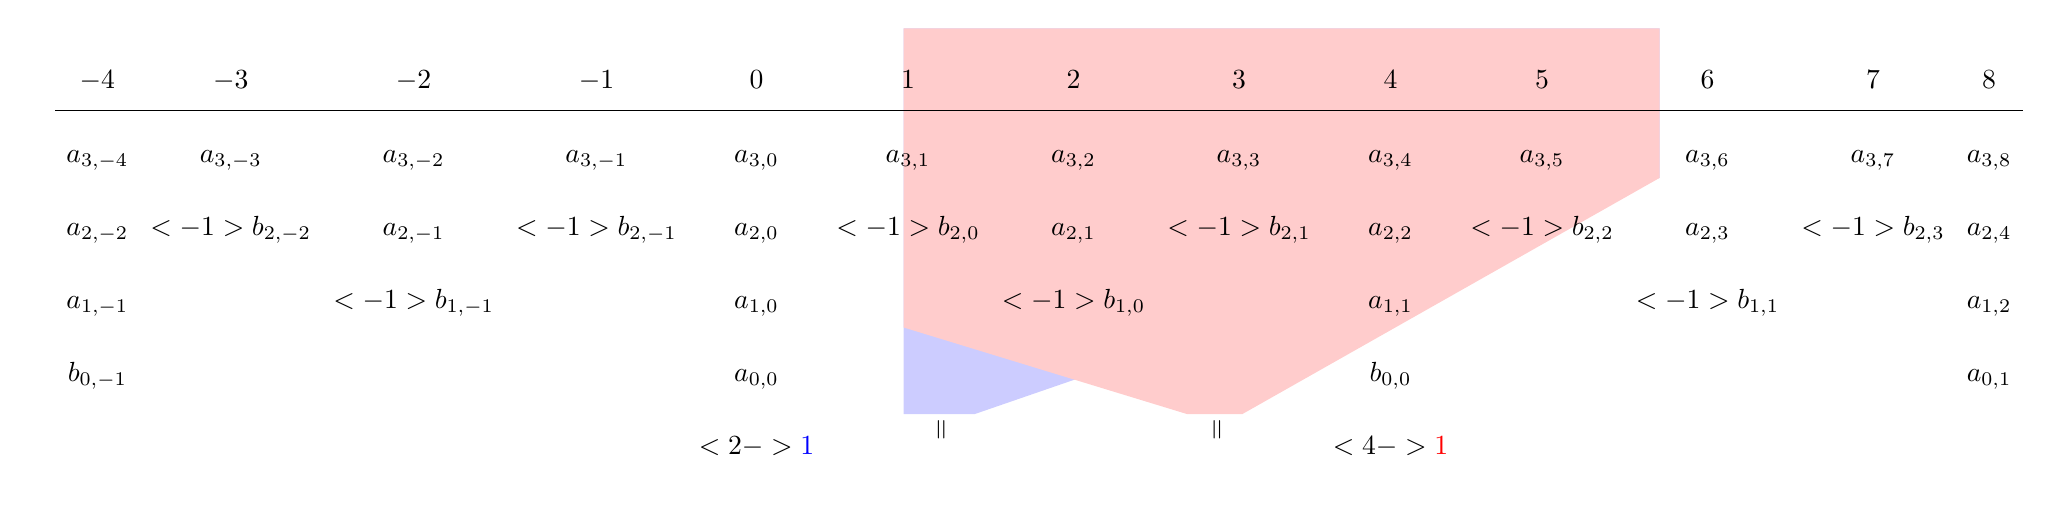
\begin{tikzpicture}[>=latex]
\uncover<3>{
\fill[color=blue!20] (-1.6,2.9)--(-1.6,-2.0)--(-0.7,-2.0)--(8,1)--(8,2.9)--cycle;
}
\uncover<5>{
\fill[color=red!20] (-1.6,2.9)--(-1.6,-0.9)--(2.0,-2.0)--(2.7,-2.0)--(8,1)--(8,2.9)--cycle;

}
\node at (0,0) {
\bgroup
\def\arraystretch{2.2}
\setlength{\tabcolsep}{4pt}
\begin{tabular}{
>{$}c<{$}
>{$}c<{$}
>{$}c<{$}
>{$}c<{$}
>{$}c<{$}
>{$}c<{$}
>{$}c<{$}
>{$}c<{$}
>{$}c<{$}
>{$}c<{$}
>{$}c<{$}
>{$}c<{$}
>{$}c<{$}
}
-4&-3&-2&-1&0&1&2&3&4&5&6&7&8
\\
\hline
a_{3,-4}&a_{3,-3}&a_{3,-2}&a_{3,-1}
&a_{3,0}&a_{3,1}&a_{3,2}&a_{3,3}&a_{3,4}
&a_{3,5}&a_{3,6}&a_{3,7} &a_{3,8}
\\
a_{2,-2}&\uncover<-1>{b_{2,-2}}&a_{2,-1}&\uncover<-1>{b_{2,-1}}
&a_{2,0}&\uncover<-1>{b_{2,0}}&a_{2,1}&\uncover<-1>{b_{2,1}}
&a_{2,2}&\uncover<-1>{b_{2,2}}&a_{2,3}&\uncover<-1>{b_{2,3}}
&a_{2,4}
\\
a_{1,-1}&&\uncover<-1>{b_{1,-1}}&&
a_{1,0}&&\uncover<-1>{b_{1,0}}&&
a_{1,1}&&\uncover<-1>{b_{1,1}}&&
a_{1,2}
\\
b_{0,-1}&&&
&a_{0,0}&&&
&b_{0,0}&&&
&a_{0,1}
\\
&&&
&\uncover<2->{\color{blue}1}&&&
&\uncover<4->{\color{red}1}&&&
&
\end{tabular}
\egroup
};
\uncover<2->{\node at (-1.1,-2.2) [rotate=90] {$=$};}
\uncover<4->{\node at ( 2.4,-2.2) [rotate=90] {$=$};}
\end{tikzpicture}
\end{center}
\end{frame}

%
% db2-Haar-Wavelet
%
\begin{frame}
\frametitle{db2 -- Haar}
\begin{columns}[T]
\begin{column}{2.5cm}
Koeffizienten:
\[
\begin{aligned}
h_0&=\phantom{-}1\\
h_1&=\phantom{-}1\\[10pt]
g_0&=\phantom{-}1\\
g_1&=-1\\
\end{aligned}
\]
\end{column}
\begin{column}{9.5cm}
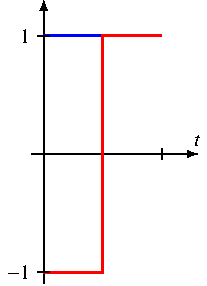
\includegraphics{../../buch/chapters/7-algo/images/db1.pdf}
\end{column}
\end{columns}
\end{frame}


\begin{frame}
\frametitle{db4}
\begin{columns}[T]
\begin{column}{2.5cm}
Koeffizienten:
\[
\begin{aligned}
h_0&=\phantom{-}0.6830127\\
h_0&=\phantom{-}1.1830127\\
h_0&=\phantom{-}0.3169873\\
h_0&=-0.1830127\\[10pt]
g_0&=\phantom{-}0.1830127\\
g_1&=-0.3169873\\
g_2&=\phantom{-}1.1830127\\
g_3&=-0.6830127
\end{aligned}
\]
\end{column}
\begin{column}{9.5cm}
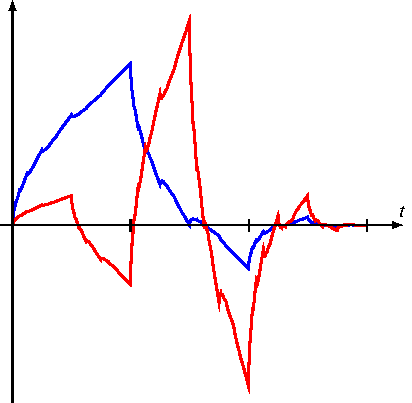
\includegraphics{../../buch/chapters/7-algo/images/db2.pdf}
\end{column}
\end{columns}
\end{frame}

\begin{frame}
\frametitle{db6}
\begin{columns}[T]
\begin{column}{2.5cm}
Koeffizienten:
\[
\begin{aligned}
h_0&=\phantom{-}0.32580343\\
h_0&=\phantom{-}1.01094572\\
h_0&=\phantom{-}0.8922014\\
h_0&=-0.03967503\\
h_0&=-0.26450717\\
h_0&=\phantom{-}0.0436163\\
h_0&=\phantom{-}0.0465036\\
h_0&=-0.01498699
\end{aligned}
\]
\end{column}
\begin{column}{9.5cm}
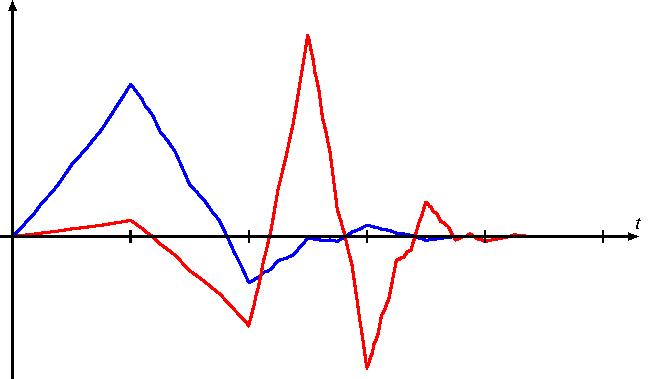
\includegraphics{../../buch/chapters/7-algo/images/db3.pdf}
\end{column}
\end{columns}
\end{frame}

\begin{frame}
\frametitle{db8}
\begin{center}
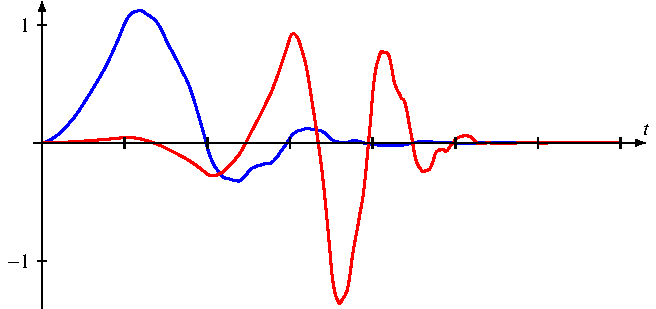
\includegraphics{../../buch/chapters/7-algo/images/db4.pdf}
\end{center}
\end{frame}

